\documentclass[sigplan,10pt,anonymous,review,screen]{acmart}

% CPP uses the ACM SIGPLAN proceedings format.  For review submissions,
% keep the review/anonymous options above.  For camera-ready, remove
% review/anonymous and fill in the ACM metadata below as instructed by ACM.

\setcopyright{none}
\settopmatter{printfolios=true,printccs=false,printacmref=false}

\acmConference[CPP 2027]{Certified Programs and Proofs}{January 2027}{Mexico City, Mexico}
\acmYear{2027}
\copyrightyear{2027}
\acmDOI{}
\acmISBN{}
%\acmSubmissionID{XXX}

\usepackage{amsmath}
\usepackage{stmaryrd}
\usepackage{booktabs}
\usepackage{tikz}
\usetikzlibrary{arrows.meta,fit,positioning}
\usepackage{../agda}

\usepackage{dsfont}
\usepackage{newunicodechar}
\newunicodechar{λ}{\ensuremath{\mathnormal\lambda}}
\newunicodechar{σ}{\ensuremath{\mathnormal\sigma}}
\newunicodechar{τ}{\ensuremath{\mathnormal\tau}}
\newunicodechar{π}{\ensuremath{\mathnormal\pi}}
\newunicodechar{ℕ}{\ensuremath{\mathbb{N}}}
\newunicodechar{∷}{\ensuremath{::}}
\newunicodechar{≡}{\ensuremath{\equiv}}
\newunicodechar{∀}{\ensuremath{\forall}}
\newunicodechar{ᴸ}{\ensuremath{^L}}
\newunicodechar{ᴿ}{\ensuremath{^R}}
\newunicodechar{ʳ}{\ensuremath{^r}}
\newunicodechar{ⱽ}{\ensuremath{^V}}
\newunicodechar{⟧}{\ensuremath{\rrbracket}}
\newunicodechar{⟦}{\ensuremath{\llbracket}}
\newunicodechar{⊤}{\ensuremath{\top}}
\newunicodechar{⊥}{\ensuremath{\bot}}
\newunicodechar{₁}{\ensuremath{_1}}
\newunicodechar{₂}{\ensuremath{_2}}
\newunicodechar{∈}{\ensuremath{\in}}
\newunicodechar{₀}{\ensuremath{_0}}
\newunicodechar{′}{\ensuremath{'}}
\newunicodechar{ˢ}{\ensuremath{^S}}
\newunicodechar{ᴬ}{\ensuremath{^A}}
\newunicodechar{∘}{\ensuremath{\circ}}
\newunicodechar{𝟙}{\ensuremath{\mathds{1}}}  
\newunicodechar{𝟘}{\ensuremath{\mathds{O}}}
% \newunicodechar{𝟙}{\ensuremath{\mathbb{I}}}  
% \newunicodechar{𝟘}{\ensuremath{\mathbb{O}}}
\newunicodechar{ᴾ}{\ensuremath{^P}}
\newunicodechar{ᶠ}{\ensuremath{^F}}
\newunicodechar{ᵀ}{\ensuremath{^T}}
\newunicodechar{⊎}{\ensuremath{\uplus}}
\newunicodechar{ι}{\ensuremath{\iota}}
\newunicodechar{⇐}{\ensuremath{\Leftarrow}}
\newunicodechar{⇒}{\ensuremath{\Rightarrow}}
\newunicodechar{∎}{\ensuremath{\mathnormal\blacksquare}}
\newunicodechar{➙}{\ensuremath{\to^P}}
\newunicodechar{Δ}{\ensuremath{\Delta}}
\newunicodechar{∅}{\ensuremath{\emptyset}}
\newunicodechar{⁺}{\ensuremath{^+}}
\newunicodechar{𝕏}{\ensuremath{\mathbb{X}}}


\newcommand{\PRNat}{\ensuremath{\mathsf{PR\mbox{-}NAT}}}
\newcommand{\PRFO}{\ensuremath{\mathsf{PR\mbox{-}FO}}}
\newcommand{\PRHO}{\ensuremath{\mathsf{PR\mbox{-}HO}}}
\newcommand{\PRFOF}{\ensuremath{\mathsf{PR\mbox{-}FO_F}}}
\newcommand{\PRHOF}{\ensuremath{\mathsf{PR\mbox{-}HO_F}}}
\newcommand{\AgdaFile}[1]{\texttt{#1}}

\begin{document}

\title{Primitive Recursion in Point-Free Categorical Calculi, Mechanized in Agda}

% Review mode is anonymous.  Keep author data commented until camera-ready.
%
% \author{Max Hertenstein}
% \affiliation{
%   \institution{University of Freiburg}
%   \country{Germany}}
%
% \author{Hannes Saffrich}
% \affiliation{
%   \institution{University of Freiburg}
%   \country{Germany}}
%
% \author{Jeremy Siek}
% \affiliation{
%   \institution{Indiana University Bloomington}
%   \country{USA}}
%
% \author{Peter Thiemann}
% \affiliation{
%   \institution{University of Freiburg}
%   \country{Germany}}
%
% \author{Philip Wadler}
% \affiliation{
%   \institution{The University of Edinburgh}
%   \country{United Kingdom}}

\begin{abstract}
Primitive recursion is usually introduced as a class of total functions
on natural numbers, but the same idea extends to richer inductive data
and higher-order programs.  We present an Agda formalization of
primitive recursion in categorical terms, using point-free first-order
and higher-order calculi, together with equational theories, setoid
models, interpretation soundness, verified translations between
paramorphism-primitive and fold-primitive presentations, and
representative instances for natural numbers, words, trees, and
many-sorted signatures.

The formalization is organized around small core calculi.  Each hom-set
is equipped with a setoid equality containing the categorical laws,
product and coproduct laws, functoriality and strength laws, and
recursion computation and uniqueness principles.  Higher-order calculi
add exponentials and their beta/eta laws.  We use setoids rather than
quotients and keep categorical distributivity as standard infrastructure:
primitive in the first-order presentation and derived from exponentials
in the higher-order presentation.

All definitions and proofs are checked by Agda using the safe fragment.
\end{abstract}

\begin{CCSXML}
<ccs2012>
 <concept>
  <concept_id>10003752.10010124.10010125.10010130</concept_id>
  <concept_desc>Theory of computation~Type theory</concept_desc>
  <concept_significance>500</concept_significance>
 </concept>
 <concept>
  <concept_id>10003752.10003790.10011740</concept_id>
  <concept_desc>Theory of computation~Categorical semantics</concept_desc>
  <concept_significance>500</concept_significance>
 </concept>
 <concept>
  <concept_id>10011007.10011006.10011041.10011047</concept_id>
  <concept_desc>Software and its engineering~Formal software verification</concept_desc>
  <concept_significance>300</concept_significance>
 </concept>
</ccs2012>
\end{CCSXML}

\ccsdesc[500]{Theory of computation~Type theory}
\ccsdesc[500]{Theory of computation~Categorical semantics}
\ccsdesc[300]{Software and its engineering~Formal software verification}

\keywords{primitive recursion, Agda, mechanized metatheory, categorical semantics, inductive types, setoids}

\maketitle

\section{Introduction}
\label{sec:introduction}

State the problem and the contribution for a CPP audience:
mechanized metatheory for primitive recursion in categorical terms,
formalized in Agda~\cite{DBLP:conf/afp/Norell08} through point-free
calculi, with a checked artifact and explicit correspondence between
the paper and Agda modules.

\paragraph{Contributions.}
\begin{itemize}
\item Categorical, point-free core calculi for first-order and
  higher-order primitive recursion.
\item Equational theories with setoid equality on hom-sets.
\item Models and interpretation soundness for paramorphism-
  primitive and fold-primitive presentations.
\item Formal translations between paramorphism-primitive and
  fold-primitive calculi, including equation preservation and round
  trips up to the equational theory.
\item Verified instance translations for natural numbers, words, trees,
  and many-sorted signatures.
\end{itemize}

\begin{figure*}
\centering
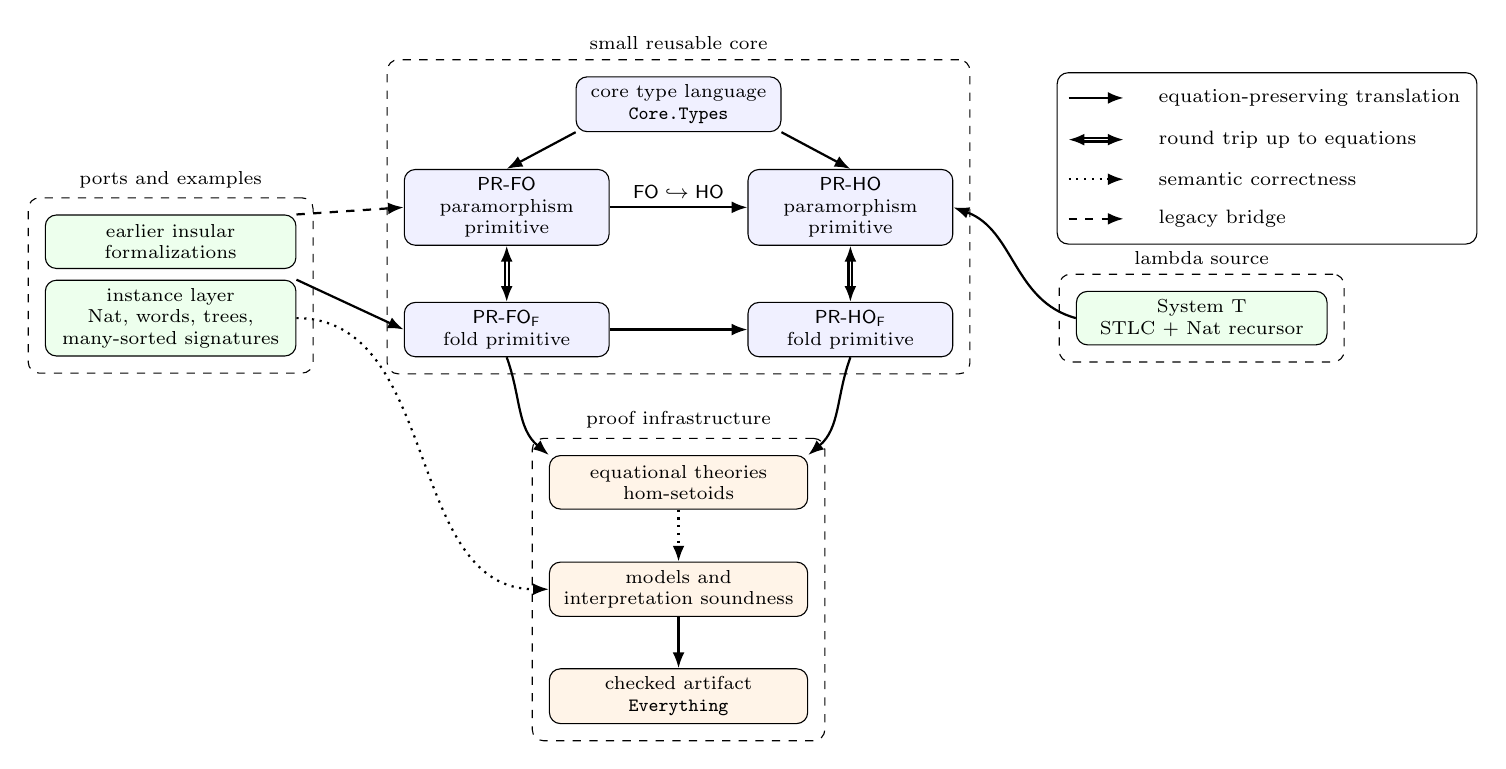
\begin{tikzpicture}[
  font=\scriptsize,
  scale=0.970,
  transform shape,
  node distance=5mm and 6mm,
  box/.style={
    draw,
    rounded corners,
    align=center,
    inner xsep=4pt,
    inner ysep=3pt,
    minimum height=7mm,
    fill=white
  },
  core/.style={box, fill=blue!6, text width=24mm},
  inst/.style={box, fill=green!7, text width=30mm},
  model/.style={box, fill=orange!9, text width=31mm},
  group/.style={draw, rounded corners, inner sep=6pt, dashed},
  preserve/.style={-{Latex[length=2mm]}, thick},
  equiv/.style={{Latex[length=2mm]}-{Latex[length=2mm]}, thick, double},
  semantic/.style={-{Latex[length=2mm]}, thick, dotted},
  bridge/.style={-{Latex[length=2mm]}, thick, dashed}
]

\node[core] (types) at (0,0) {core type language\\\AgdaFile{Core.Types}};
\node[core] (prfo) at (-2.25,-1.35) {\PRFO{}\\paramorphism primitive};
\node[core] (prho) at (2.25,-1.35) {\PRHO{}\\paramorphism primitive};
\node[core] (prfof) at (-2.25,-2.95) {\PRFOF{}\\fold primitive};
\node[core] (prhof) at (2.25,-2.95) {\PRHOF{}\\fold primitive};

\node[inst] (legacy) at (-6.65,-1.8) {earlier insular\\formalizations};
\node[inst] (instances) at (-6.65,-2.8) {instance layer\\Nat, words, trees,\\many-sorted signatures};
\node[inst] (systemt) at (6.85,-2.8) {System T\\STLC + Nat recursor};

\node[model] (eqs) at (0,-4.95) {equational theories\\hom-setoids};
\node[model] (models) at (0,-6.35) {models and\\interpretation soundness};
\node[model] (artifact) at (0,-7.75) {checked artifact\\\AgdaFile{Everything}};

\node[group, fit=(types) (prfo) (prho) (prfof) (prhof),
  label={[font=\scriptsize]above:small reusable core}] {};
\node[group, fit=(legacy) (instances),
  label={[font=\scriptsize]above:ports and examples}] {};
\node[group, fit=(systemt),
  label={[font=\scriptsize]above:lambda source}] {};
\node[group, fit=(eqs) (models) (artifact),
  label={[font=\scriptsize]above:proof infrastructure}] {};

\draw[preserve] (types.south west) -- (prfo.north);
\draw[preserve] (types.south east) -- (prho.north);
\draw[preserve] (prfo.east) -- node[above=2pt, fill=white, inner sep=1pt] {$\mathsf{FO}\hookrightarrow\mathsf{HO}$} (prho.west);
\draw[equiv] (prfo.south) -- (prfof.north);
\draw[equiv] (prho.south) -- (prhof.north);
\draw[preserve] (prfof.east) -- (prhof.west);

\draw[preserve] (systemt.west) to[out=165,in=-20] (prho.east);
\draw[bridge] (legacy.north east) -- (prfo.west);
\draw[preserve] (instances.north east) -- (prfof.west);
\draw[semantic] (instances.east) to[out=0,in=180] (models.west);

\draw[preserve] (prfof.south) to[out=-70,in=140] (eqs.north west);
\draw[preserve] (prhof.south) to[out=-110,in=40] (eqs.north east);
\draw[semantic] (eqs.south) -- (models.north);
\draw[preserve] (models.south) -- (artifact.north);

\matrix[draw, rounded corners, anchor=north west, column sep=3mm,
  row sep=1mm, inner sep=3pt, font=\scriptsize] (legend) at (4.95,0.42) {
  \draw[preserve] (0,0) -- +(7mm,0); &
    \node[anchor=west] {equation-preserving translation}; \\
  \draw[equiv] (0,0) -- +(7mm,0); &
    \node[anchor=west] {round trip up to equations}; \\
  \draw[semantic] (0,0) -- +(7mm,0); &
    \node[anchor=west] {semantic correctness}; \\
  \draw[bridge] (0,0) -- +(7mm,0); &
    \node[anchor=west] {legacy bridge}; \\
};

\end{tikzpicture}
\caption{Overview of the mechanized contribution.  The new core
calculi factor out common syntax, equations, models, and translation
proofs.  Instance modules connect System~T and the earlier
single-purpose formalizations to the core, while arrow styles record
the formal property proved about each connection.  The fold-level
FO-to-HO arrow is derived via the P/F equivalences.}
\Description{A diagram with a reusable core in the upper middle, a
legend in the upper right aligned with the top of the core, ports and
examples to the left of the core, a separate System T source box below
the legend with its dashed group bottom aligned with the bottom of the
core, and proof infrastructure centered below the core.  The System T
box has a direct arrow into PR-HO.  Solid, double, dotted, and dashed
arrows distinguish equation-preserving translations, equivalences up to
equations, semantic correctness theorems, and legacy bridges.  The
fold-level FO-to-HO arrow is derived by composing the
paramorphism/fold equivalences with the first-order to higher-order
embedding.}
\label{fig:contribution-overview}
\end{figure*}

\section{Overview of the Formalization}
\label{sec:overview}

Use this section to orient reviewers before presenting details.  Include
a table mapping paper claims to Agda modules.

\begin{table}
\caption{Draft paper-to-artifact map.}
\label{tab:artifact-map}
\begin{tabular}{ll}
\toprule
Paper component & Agda modules \\
\midrule
Core type language & \AgdaFile{Core.Types} \\
\PRFO{} syntax and equations & \AgdaFile{Core.PRFO}, \AgdaFile{Core.Equations.PRFO} \\
\PRHO{} syntax and equations & \AgdaFile{Core.PRHO}, \AgdaFile{Core.Equations.PRHO} \\
Fold-primitive presentations & \AgdaFile{Core.PRFOFold}, \AgdaFile{Core.PRHOFold} \\
Models and soundness & \AgdaFile{Core.Models.*} \\
Hom-setoid packaging & \AgdaFile{Core.Models.Setoids.*} \\
P/F interdefinability & \AgdaFile{Core.Translations.*ParamorphismFold} \\
FO to HO translation & \AgdaFile{Core.Translations.PRFOToPRHO} \\
System T to PR-HO & \AgdaFile{Core.Instances.SystemT} \\
Instances & \AgdaFile{Core.Instances.*} \\
Trusted entry point & \AgdaFile{Everything} \\
\bottomrule
\end{tabular}
\end{table}

\section{Core Calculi}
\label{sec:core-calculi}

Describe the type grammar, point-free terms, products, coproducts,
exponentials, functorial action, strength, folds, and paramorphisms.
Make clear which operators are primitive in each presentation.

\section{Equational Theories and Setoid Models}
\label{sec:equations-models}

Explain why the formalization uses generated equality relations and
model-level setoids rather than quotients.  State the key classes of
laws:
category laws, product/coproduct beta-eta laws, exponential beta-eta
laws for higher order, functor/strength laws, distributivity laws, and
recursion beta/uniqueness laws.

\section{Paramorphisms and Folds}
\label{sec:paramorphisms-folds}

Present the two primitive choices:
paramorphism primitive (\(P\)) and fold primitive (\(F\)).  State the
formal interdefinability theorem:
translations in both directions preserve equations and compose to the
identity up to the appropriate equational theory.

\section{Instances}
\label{sec:instances}

Summarize the verified instances: natural numbers, finite alphabets and
words, trees, and many-sorted signatures.  Explain the semantic
correctness statements and representation theorems.

\section{Formalization Design}
\label{sec:formalization-design}

CPP reviewers usually expect design tradeoffs.  Discuss:
\begin{itemize}
\item intrinsic syntax versus contextual syntax;
\item setoids instead of quotients;
\item strictly positive descriptions/containers for inductive types;
\item guardedness and finitary fragments;
\item why distributivity is treated as infrastructure, not novelty;
\item safe Agda checking and the role of \AgdaFile{Everything.agda}.
\end{itemize}

\section{Related Work}
\label{sec:related-work}

Position the work relative to primitive recursion, System~T, categorical
semantics, mechanized metatheory, Agda formalizations of syntax with
binders, and libraries for containers or W-types.

\section{Conclusion}
\label{sec:conclusion}

State what is now mechanically established and what remains future work:
generic refactoring of the FO/HO P/F proof, richer instance libraries,
and further categorical semantics.

\begin{acks}
% Acknowledgments are usually omitted or anonymized during review.
\end{acks}

\bibliographystyle{ACM-Reference-Format}
\bibliography{../jfprefs}

\end{document}
